\documentclass[ruledheader,noindentfirst,anapcustomindent,abntfigtabnum,tocpage=plain]{abnt}

\usepackage{amsmath, amssymb, amsthm, verbatim, amsfonts, amstext}
%\usepackage[latin1]{inputenc}
\usepackage[brazilian]{babel}
\usepackage[utf8]{inputenc}
\usepackage[T1]{fontenc}
\usepackage{dropping}
\usepackage{graphicx}
\usepackage[hang,small,bf]{caption}
\usepackage[abnt-etal-list=0,abnt-etal-text=it,abnt-and-type=&,abnt-emphasize=bf,abnt-full-initials=yes,alf,bibjustif]{abntcite}
\usepackage{fancyhdr}
\usepackage{makeidx}
\usepackage[none]{hyphenat}
\usepackage{color}
\usepackage{subfig}
\usepackage{algorithms}
\usepackage{algorithmic}
\usepackage{mdwlist}
\usepackage{bm}
\usepackage[titletoc,title]{appendix}
\usepackage{ltxtable}
\usepackage{longtable}
\usepackage{supertabular}
\usepackage{indentfirst}
\usepackage{color}
\usepackage{icomma}
\usepackage{url}

\usepackage{float}
\usepackage{multirow}
\usepackage{longtable}
\usepackage{enumerate}
\sloppy

%
%Tradução do pacote Algorithm para portugues
%
\renewcommand{\algorithmicrequire}{\textbf{Entrada:}}
\renewcommand{\algorithmicensure}{\textbf{Saída:}}
\renewcommand{\algorithmicend}{\textbf{fim}}
\renewcommand{\algorithmicif}{\textbf{se}}
\renewcommand{\algorithmicthen}{\textbf{então}}
\renewcommand{\algorithmicelse}{\textbf{senão}}
\renewcommand{\algorithmicelsif}{\algorithmicelse \, \algorithmicif}
\renewcommand{\algorithmicendif}{\algorithmicend \, \algorithmicif}
\renewcommand{\algorithmicfor}{\textbf{para}}
\renewcommand{\algorithmicforall}{\textbf{para todo}}
\renewcommand{\algorithmicdo}{\textbf{fazer}}
\renewcommand{\algorithmicendfor}{\algorithmicend \, \algorithmicfor}
\renewcommand{\algorithmicwhile}{\textbf{enquanto}}
\renewcommand{\algorithmicendwhile}{\algorithmicend \, \algorithmicwhile}
\renewcommand{\algorithmicloop}{\textbf{laço}}
\renewcommand{\algorithmicendloop}{\algorithmicend \, \algorithmicloop}
\renewcommand{\algorithmicrepeat}{\textbf{repetir}}
\renewcommand{\algorithmicuntil}{\textbf{até}}
\renewcommand{\algorithmiccomment}[1]{\{#1\}}
\renewcommand{\listalgorithmname}{Lista de Algoritmos}
\floatname{algorithm}{Algoritmo}
%%%%%%%%%%%%%%%%%%%%%%%%%%%%%%%%%%%%%%%%%%%%%%%%%%%%%%%%%%%%%%%%%%%%%%%%%%%%%%%%%%%
\newcommand*\rot{\rotatebox{90}}
\newcommand*\V{\ding{51}}
\newcommand\tab[1][1cm]{\hspace*{#1}}

\makeindex

%%%% O arquivo estiloCAP.tex possui as definições para ciação do estilo de capítulo (fonte de título, barras horizontais, etc.)
% ele não gera texto de saída, é um arquivo de configuração somente
%
% \input{configuracao/estiloCAP}
%%%%%%%%%%%%%%%%%%%%%%%%%%%%%%%%%%%%%%%%%%%%%%%FIM DO PREAMBULO%%%%%%%%%%%%%%%%%%%%%%%%%%%%%%%%%%%%%%%%%%%%%%%%%%%%%%%%%%%%%%%%%%





\begin{document}

%%%%% IMPORTANTE: ALTERA O TEXTO ENTRE ARIAL E TIMES NEW ROMAN (ALTERNAR OS COMENTÁRIOS)
%
%%%%%%%%%%%%%%%%%%%%%PARA UTILIZAR ARIAL%%%%%%%%%%%%%%%%%%%%%%%
%
\fontfamily{phv}                    %fonte Arial
\renewcommand{\rmdefault}{phv}      %
%
%%%%%%%%%%%%%%%%%%%%%PARA UTILIZAR TIMES%%%%%%%%%%%%%%%%%%%%%%%
%
%\fontfamily{ptm}               %fonte Times
%\renewcommand{\rmdefault}{ptm} %
%
%%%%%%%%%%%%%%%%%%%%%%%%%%%%%%%%%%%%%%%%%%%%%%%%%%%%%%%%%%%%%%%

%%%%%%%%%%%%%Arquivos .tex com os elementos pré-textuais
%
\thispagestyle{empty}

\vfill
 \begin{center}
    \begin{figure}[t]
     \centering
            % \includegraphics[width=5cm]{figures/logo.pdf}\\[-0.1in]
            \includegraphics[width=15cm]{figuras/logo-uit.pdf}\\[-0.1in]
     \end{figure}

    {\large\bfseries UNIVERSIDADE DE ITAÚNA} \\
    {\large\bfseries PRÓ-REITORIA DE ENSINO} \\
    {\large\bfseries COORDENAÇÃO DE CIÊNCIA DA COMPUTACAO}  \\ 
    {\large\bfseries BACHARELADO EM CIÊNCIA DA COMPUTAÇÃO}  \\ 

    \vspace*{1in}
    \begin{large} \bfseries Eugênio Cunha\end{large}\\[0.4in]

    \vspace*{4cm}
    \noindent \\
    \large\bfseries{APRENDIZADO DE MÁQUINA APLICADO À VALORAÇÃO DAS COMPETÊNCIAS DE UMA REDAÇÃO} \\
    \vfill
    \large\bfseries{ ITAÚNA \\ 2017}
\end{center}

\normalsize
\begin{titlepage}
\vfill
\begin{center}

    {\large EUGÊNIO CUNHA\\}
    \vspace{2cm}
    {\Large \textsc{APRENDIZADO DE MÁQUINA APLICADO À VALORAÇÃO DE REDAÇÕES}\\}
    \vspace{1cm}
    \hspace{.45\linewidth}
    \begin{minipage}{.50\linewidth}

            Projeto submetido à Coordenadoria do Curso de Bacharelado 
            em Ciência da Computação da Universidade de Itaúna - Campus Verde, como requisito 
            parcial para obtenção do grau de Bacharel em Ciência da Computação.

            \vspace{0.5 cm}

            Área de pesquisa: Aprendizagem de Máquina

            \vspace{0.5 cm}

            Orientador: Prof. Dr. Marco Túlio Alves N Rodrigues
    
    \end{minipage}

    \vspace{2cm}
    \vfill
    {\large Itaúna\\ 2017}
\end{center}

\end{titlepage}
\begin{folhadeaprovacao}
\setlength{\ABNTsignthickness}{0.2pt}
\setlength{\ABNTsignskip}{1.7cm}

\begin{center}
\includegraphics[width=2.5cm]{figuras/brasao_uit.pdf}\\
            {UNIVERSIDADE DE ITAÚNA} \\
            {COORDENAÇÃO DE CIÊNCIA DA COMPUTAÇÃO}  \\

    \vspace{1.5cm}
                                    {EUGÊNIO CUNHA}\\
    \bfseries{}
\end{center}

Este projeto foi julgada adequada para a obten\c{c}\~{a}o do Grau de Bacharel em Ciência da Computação, sendo aprovada pela coordenação de ciência da computação do curso de Bacharelado em Ciência da Computação
do Campus verde da Universidade de Itaúna e pela banca examinadora:

    \vspace{0.15cm}
    \assinatura{Orientador: Prof. Dr. Marco Túlio Alves N Rodrigues\\ Universidade de Itaúna- UIT}
    \assinatura{Avaliador: Prof. Me. Felipe Domingos da Cunha \\ Universidade de Itaúna- UIT}
    \vspace{0.15cm}%\vfill

    \begin{center}
        Itaúna, 19 de Junho de 2017
    \end{center}
\end{folhadeaprovacao}
\vspace*{15cm}

\hfill Dedico este trabalho ao meu filho Davi, sempre preocupado em proporcionar um minuto de brincadeira durante minhas horas de trabalho, ``meus melhores minutos''! \\
\include{pre-textuais/agradecimentos}
%\thispagestyle{empty}


\begin{flushright}
\begin{minipage}[r]{10cm}
\vspace{18cm}
``Os computadores são incrivelmente rápidos, precisos e burros; os homens são incrivelmente lentos, imprecisos e brilhantes; juntos, seus poderes ultrapassam os limites da imaginação''.
\begin{flushright}
Albert Einstein
\end{flushright}
\end{minipage}
\end{flushright}
\pagestyle{plain}%%%%% Utilizar ESTILO PLAIN AQUI%%%%%%%
\chapter*{Resumo}

\noindent Este trabalho baseou-se no estudo da avalição de uma redação que é a 
soma de um conjunto de competências exigidas em um texto do tipo 
dissertativo-argumentativo com temas diversificados de ordem social, 
científica, cultural ou política. Fundamentou-se no estudo das técnicas de 
aprendizado de máquina supervisionado que provê uma gama diversificada de 
algoritmos poderosos para classificações de textos.

O objetivo deste trabalho é classificar as competências exigidas em um texto de 
redação a partir do treinamento de um algoritmo de aprendizado de máquina com
base em um \textit{corpus} de redações avaliadas seguindo as competências exigidas em 
uma redação do tipo dissertativa-argumentativa.


% A extração de Informação compreende técnicas e algoritmos que realisam 
% duas tarefas importantes: a identificação de informações desejadas a partir de documentos estruturados e não-estruturados, e o arm
% azenamento dessas informações em um formato apropriado para uso futur
o.
% O \textit{corpus} de redações avaliadas foi minerada de banco de redações manti

Palavras-chaves: Aprendizado de máquina, Redação, Classificação, Orange3
    
\include{pre-textuais/abstract}

%%%Comandos para criação automática das listas
%
\tableofcontents
\listoffigures
\listoftables

%%%Comandos para criar outras listas não suportadas pelo pacote ABNTex%%%
%
% \pretextualchapter{Lista de Símbolos}
\begin{basedescript}{\desclabelstyle{\pushlabel}\desclabelwidth{6em}}
\item[$TAG$] Rótulo%
\item[$BOW$] Representação da frequência acumulada de palavras em documentos
diferentes a partir de um dicionário pré-­criado%

\end{basedescript}
\newpage

\pretextualchapter{Lista de Abreviações}
\begin{basedescript}{\desclabelstyle{\pushlabel}\desclabelwidth{6em}}
\item[{CEBRASPE}] Centro Brasileiro de Pesquisa em Avaliação e Seleção e de Promoção de Eventos%
\item[{CSF}] Ciência sem fronteiras%
\item[{ENEM}] Exame Nacional do Ensino Médio%
\item[{HTML}] \textit{HyperText Markup Language}%
\item[{IA}] Inteligência artificial%
\item[{INEP}] Instituto Nacional de Estudos e Pesquisas Educacionais%
\item[{SISU}] Sistema de Seleção Unificada%
\item[{UNB}] Universidade de Brasília%
\item[{JSON}] \textit{JavaScript Object Notation}%
\end{basedescript}
\newpage
%%%%%%%%%%%%%%%%%%%%%%%%%%%%%%%%%%%%%%%%%%%%%%%%%%%%%%%%%%%%%%%%%%%%

%Capítulos passam a ter páginas numeradas
%
\pagestyle{fancy}

%resseta os contadores de capítulo e seção
%
\renewcommand{\chaptermark}[1]{\markboth{#1}{}}
\renewcommand{\sectionmark}[1]{\markright{\thesection\ #1}}

%%% Outros arquivos .tex. É acoselhável utilizar vários arquivos, pelo menos um por capítulo
\chapter{Introdução}\label{CAP:introducao}

\noindent O desenvolvimento de uma redação e uma atividade prática presente na cultura civilizada desde a invenção da escrita.
Já faz pelo menos uma década que um bom desempenho na redação do Exame Nacional de Ensino Médio - ENEM  virou sinônimo de chances maiores para ser aprovado no processo seletivo de acesso a inúmeras universidades públicas ~\cite{sisu:2017} e a importantes programas de governo como Ciência sem fronteiras ~\cite{csf:2017}.

Em todo processo seletivo é comum o uso de marcações em gabaritos afim de automatizar o processo de correção, uma alternativa rápida e segura, até mesmo aplicações de provas eletrônicas são cada vez mais comum. Um exemplo seria o processo seletivo para avaliador das redações do ENEM que durante a ``FASE II'' respondem uma prova eletrônica eliminatória ~\cite{paq_a:2016}. É notável que todo o processo evoluiu com objetivo de agilidade, confiança e segurança do resultado, entretanto a avaliação das competências de uma redação ainda depende exclusivamente da supervisão de duas ou mais pessoas envolvidas ~\cite{edital_enem:2016}.

A redação é aplicada no ENEM desde a primeira edição 1998, hoje o maior exame do Brasil, que na edição de 2016 teve 8.627.195 escritos confirmados, e a participação direta de 11.360 profissionais externos na correção de 5.825.134 redações, entre eles, 378 supervisores e 10.982 avaliadores de acordo com a CEBRASPE ~\cite{relatorio_de_gestao:2016}. 

Segundo o edital do ENEM 2016 ~\cite{edital_enem:2016} cada redação foi avaliada por, pelo menos, dois avaliadores, de forma independente, contabilizando um número mínimo de 11.650.268 avaliações manuais, das competências exigidas em um texto de redação pelo ENEM.

\textit{Machine Learning} ou aprendizado de máquina é uma área de IA cujo objetivo é o desenvolvimento de técnicas computacionais sobre o aprendizado bem como a construção de sistemas capazes de adquirir conhecimento de forma automática. Os algoritmos de aprendizado de máquina procuram padrões dentro de um conjunto de dados~\cite{machine_learning:1997}. Esses algoritmos existem há bastante tempo, uma ciência que não é nova, mas que está ganhando um novo impulso enquanto o processamento computacional cresce e fica mais barato.

A hipótese desta monografia é que um ou mais modelos de aprendizado de máquina na valoração das competências de uma redação pode ser tão eficiênte quanto o processo de avaliação manual.

\section{Definição do Problema de Pesquisa}

Dado um corpus de redações avaliar as competências exigidas em um texto de redação do tipo dissertativo-argumentativo substituindo a etapa de avaliação manual.

\section{Motivação}

Com crescente volume e variedade de dados disponíveis, o processamento computacional que está mais barato e mais poderoso, e o armazenamento de dados de forma acessível, o aprendizado de máquina está no centro de muitos avanços tecnológicos atingindo áreas antes exclusivas de seres humanos. Os carros autônomos do Google são o exemplo de uma atividade antes exclusiva de um humano e hoje exercida e aperfeiçoada por algoritmos de aprendizado de máquina ~\cite{waymo:2017}.

Aplicações de aprendizado de máquina estão presentes na nossa vida cotidiana como, resultados de pesquisa web, análise de sentimento baseado em texto e na detecção de fraudes em operações com cartões de crédito ~\cite{batista1999aplicando}.

As competências exigidas em uma redação podem ser avaliadas por aprendizado de máquina, diferente de um ser humano um algoritmo de aprendizado de máquina está livre de ansiedade, fadiga, \textit{stress} entre outro fatores emocionais que afetão uma avaliação imparcial a opinião do autor.

\section{Objetivos Gerais e Específicos}

Este trabalho tem como objetivo geral aplicar aprendizado de máquina na avaliação das competências exigidas em um texto de redação do tipo dissertativo-argumentativo.

\subsection{Objetivos Especificos}

O método de construção do conhecimento deste trabalho terá como fundamentos processos de pesquisas relacionadas às áreas descritas. O mesmo será dividido em etapas dentro do escopo geral de forma detalhada e refinada para alcançar o objetivo geral acima, são particularizadas como os seguintes objetivos específicos:

\begin{itemize}
 \item Percorrer o banco de redações UOL ~\cite{uol_banco_redacoes:2017} em páginas HTML, filtrar e coletar redações avaliadas;
 \item Normalizar os textos coletados, separar o tema, título, texto e competências avaliadas em uma estrura no formato JSON;
 \item Montar um fluxo de trabalho utilizando a ferramenta para mineração de dados \textit{Orange} ~\cite{JMLR:demsar13a} com modelos classificadores de multiplas classes;
 \item Ajustar e treinar os modelos classificadores com o corpus de redações; 
 \item Realizar testes de acurácia, \textit{overfitting} e \textit{noise} sobre os classificadores;
 \item Representar e comparar graficamente os resultados obtidos. 
\end{itemize}

\section{Contribuições}

O presente estudo contribuirá na área do aprendizado de máquina e diretamente no processo de avaliação de um texto em prosa do tipo dissertativo argumentativo.

\section{Organização do trabalho}

\noindent \textbf{Capitulo \ref{trab_rela}}: Trabalhos Relacionados cita alguns dos trabalhos lidos para  embasamento teórico que serviram de base para solucionar o problema proposto.

\noindent \textbf{Capitulo \ref{meto}}: Método proposto apresenta as etapas passo a passo para desenvolver e resolver o problema proposto deste trabalho.

\noindent \textbf{Capitulo \ref{desen}}: Desenvolvimento descreve cada procedimento metodológico que será
utilizado para a realização da pesquisa.

\noindent \textbf{Capitulo \ref{result}}: Resultados Experimentais apresenta os resultados obtidos do trabalho desta pesquisa.
\chapter{Trabalhos Relacionados}\label{trab_rela}

% \section{Ferramentas para mineração de dados}

% \section{Modelo emsemble}

% \section{Modelo boost}

% \section{Modelo adaboost}


\chapter{Fundamentação Teórica}\label{fund_teo}

Este capítulo irá abordar alguns conceitos que serão necessários durante o desenvolvimento
deste trabalho para que o projeto tenha fundamentos concretos.

\section{Processamento de linguagem natural}

O desenvolvimento de modelos computacionais para a realização de tarefas que dependem de informações expressas em uma língua natural também conhecido como processamento de linguagem natural, cresce desde o início da década de 1990, segundo ~\cite{vieira2010processamento} "o crescimento da internet e a profusão de textos disponíveis direcionaram os esforços do PLN para o tratamento de textos mais do que para o discurso falado". Ainda segundo o autor neste mesmo período iniciou as pesquisas sobre conjuntos de textos sobre um domínio de conhecimento onde cada uma das suas palavras foram identificadas segundo sua função sintática.

O processamento de linguagem natural segundo o trabalho de ~\cite{teixeira2011analise} pode envolver diversas etapas: \textit{tokenizer} ou divisão do texto em termos mais simples, \textit{phrase chunking} ou análise sintática e \textit{part-of-speech tagging} ou identificação da classe gramatical das palavras. Existem também outras etapas mais específicas, como a identificação de entidades (datas, nomes, número, etc), entretanto algumas destas etapas são essenciais para o processamento correto do texto, como o \textit{tokenizer}.    

\section{\textit{Bag of words}}

Segundo ~\cite{alexandra_alves:2010} o BOW (\textit{Bag of Words}) é o modelo mais utilizado em aplicações de classificação de texto. Com baixo custo em termos de processamento este modelo transforma a cadeia de caracteres de um documento num conjunto de palavras, registrando além da presença de uma palavra, a sua frequência.

Entretanto ainda segundo o autor, propriedades básicas do texto, como a ordem em que as palavras ocorrem e a pontuação, são ignoradas, além da incapacidade em capturar a semântica do texto, isto é, há palavras com significados distintos que apesar de serem exatamente iguais têm significados diferentes, dependendo do contexto em que são utilizadas.

Obviamente, termos que aparecem em todos os documentos são denominados \textit{stop words} e não serão analisados, geralmente são os pronomes, artigos e as preposições. Estes termos não são úteis, visto que têm uma semântica fraca e somente desempenham um papel funcional no texto. Para melhorar os métodos de processamento normalmente são removidas, em vários casos a remoção das \textit{stop words} não traz consequências graves segundo o autor.

Na Tabela ~\ref{tab:bow}, \textbf{w}\textsubscript{i} representa uma palavra, \textbf{d}\textsubscript{j} representa um documento e \textbf{p}\textsubscript{ij} o peso atribuído a cada palavra no documento.

\begin{longtable}{|c|c|c|c|c|c|}
    \caption{Modelo \textit{Bag of Words} é maneira mais comum de representar coleções de documentos no qual cada documento é representado por um vetor e cada palavra da coleção representa uma dimensão do vetor.}
    \label{tab:bow}
    \endfirsthead
    \multicolumn{6}{l}%
    {Tabela \thetable{} (continuação)}
    \endhead
    \multicolumn{6}{l}%
    {Continua na próxima página}\\
    \endfoot
    \endlastfoot
    \hline  & \textbf{w}\textsubscript{1} & \textbf{w}\textsubscript{2} & \textbf{w}\textsubscript{3} & \textbf{w}\textsubscript{...} & \textbf{w}\textsubscript{n} \\
    \hline \textbf{d}\textsubscript{1} & p\textsubscript{11} & p\textsubscript{12} & p\textsubscript{13} & p\textsubscript{...} & p\textsubscript{1n} \\
    \hline \textbf{d}\textsubscript{2} & p\textsubscript{21} & p\textsubscript{22} & p\textsubscript{23} & p\textsubscript{...} & p\textsubscript{2n} \\
    \hline \textbf{d}\textsubscript{3} & p\textsubscript{31} & p\textsubscript{32} & p\textsubscript{33} & p\textsubscript{...} & p\textsubscript{3n} \\
    \hline \textbf{d}\textsubscript{4} & p\textsubscript{41} & p\textsubscript{42} & p\textsubscript{43} & p\textsubscript{...} & p\textsubscript{4n} \\
    \hline \textbf{d}\textsubscript{n} & p\textsubscript{n1} & p\textsubscript{n2} & p\textsubscript{n3} & p\textsubscript{...} & p\textsubscript{nn} \\
    \hline
\end{longtable}

Ainda segundo ~\cite{alexandra_alves:2010} existem várias medidas para calcular os valores dos pesos de p\textsubscript{ij}. Essas medidas podem ser classificadas em dois tipos distintos: baseadas em frequências e binárias. Os pesos baseados em frequência visam contabilizar o número de ocorrências de um dado termo num determinado documento, servindo como base para diversas medidas estatísticas e os pesos binários indicam a ocorrência ou não de um dado termo num determinado documento.

\section{Aprendizado de Máquina supervisionado}

De acordo com ~\cite{de2005anotaccao} no decorrer da última década, o Aprendizado de Máquina tem atestado ser uma ferramenta eficiente para realizar tarefas linguísticas, que de outro maneira seria impossível devido à enorme quantidade de mão-de-obra e tempo necessário. 

Segundo o trabalho de ~\cite{batista2003pre}, na área de Aprendizado de Máquina foram propostos diversos paradigmas aptos a aprender a partir de um conjunto de exemplos. Uma premissa básica para todos os paradigmas de Aprendizado de Máquina supervisionado é que o conceito a ser induzido deve ser referente ao caso observado, ou seja, cada exemplo deve estar denominado com a classe a qual pertence. 

Entretanto o autor cita que ``Se todos os casos são memorizados, o classificador pode se tornar lento e difícil de manusear. O ideal é reter casos prototípicos que juntos resumem toda uma informação importante.''.

\section{Classificador \textit{Adaboost}}

\textit{Boosting} é um conjunto de métodos e procedimentos de Aprendizado de Máquina que mescla vários classificadores fracos para aperfeiçoar a \textit{acurácia} geral. O algoritmo atualiza os pesos dos exemplos a cada iteração e cria um classificador adicional. Os classificadores são combinados por um esquema simples de votação. O algoritmo mais famoso baseado em Boosting é o Adaboost (Algoritmo Adaptive Boosting) que atualiza os pesos dos exemplos em que os classificadores anteriores cometeram erros, focando o classificador adicional nos exemplos mais difíceis ~\cite {duarte2009algoritmo}.

Merjildo et al. (2013) mostra as propriedades que simplificam o uso do classificador \textit{AdaBoost}. O autor cita em seu trabalho que os parâmetros empregados para analisar dados de grandes proporções e as margens entre as classes podem ser mais precisas do que em outros métodos e o custo computacional é baixo, dado que corresponde a um programa de complexidade linear e evita o uso de componentes computacionais pesados.

Por fim, este classificador escolhido para essa pesquisa, tem como objetivo reconhecer padrões complexos a partir de combinações de características simples baseadas em formas que podem estar presentes em textos de redação do tipo dissertativo-argumentativo.

\section{Métricas utilizadas}

Avaliar o desempenho de um modelo é um dos estágios principais deste estudo, a avaliação se baseia nas predições que são produzidas pelo modelo induzido. 

Na comparação dos resultados experimentais serão utilizadas sete métricas de avaliações sobre modelo supervisionado \textit{AdaBoost}, que são:

\textbf{Matriz de confusão} - A matriz de confusão de uma hipótese H oferece uma medida efetiva do modelo de classificação, ao mostrar o número de classificações corretas versus as classificações preditas para cada classe, sobre um conjunto de exemplos verdadeiros como descrito na Tabela ~\ref{tab:sample_matrix_confusion}.

\begin{table}[H]
\centering
\begin{tabular}{rc|c|c|}
\cline{3-4}
\multicolumn{2}{c|}{\multirow{2}{*}{}} & \multicolumn{2}{c|}{Valor verdadeiro} \\ \cline{3-4} 
\multicolumn{2}{c|}{} & positivos & negativos \\ \hline
\multicolumn{1}{|c|}{\multirow{2}{*}{Valor previsto}} & positivos & VP & FP \\ \cline{2-4} 
\multicolumn{1}{|c|}{} & negativos & FN & VN \\ \hline
\end{tabular}
\caption{Matriz de confusão ou tabela de contingência}
\label{tab:sample_matrix_confusion}
\end{table}

\textbf{Acurácia} - porcentagem de amostras positivas e negativas classificadas corretamente sobre a soma de amostras positivas e negativas dada pela fórmula da equação ~\ref{eq:acuracia}:
\begin{equation} \label{eq:acuracia}
 acuracia = \frac{TP+TN}{VP+VN+FP+FN}
\end{equation}

\textbf{Sensitividade} - ou \textit{recall} é a porcentagem de amostras positivas classificadas corretamente sobre o total de amostras positivas dada pela fórmula da equação ~\ref{eq:recall}:
\begin{equation} \label{eq:recall}
  sensitividade = \frac{TP}{TP+FN} = \frac{TP}{Positivo}
\end{equation}

\textbf{Precisão} - ou \textit{precision} é a porcentagem de amostras positivas classificadas corretamente sobre o total de amostras classificadas como positivas dada pela fórmula da equação ~\ref{eq:precision}:
\begin{equation} \label{eq:precision}
    precisao = \frac{TP}{TP+FP}
\end{equation}

\textbf{Especificidade} - ou \textit{specificity} é a porcentagem de amostras negativas identificadas corretamente sobre o total de amostras negativas dada pela fórmula da equação ~\ref{eq:specificity}:
\begin{equation} \label{eq:specificity}
    especificidade = \frac{TN}{TN+FP}=\frac{TN}{Negativo}
\end{equation}

\textbf{\textit{F1}} - ou \textit{F-Measure} é uma média ponderada de precisão e sensitividade dada pela fórmula da equação ~\ref{eq:fscore}:
\begin{equation} \label{eq:fscore}
    f1=\frac{2*(precisao*sensitividade)}{precisao+sensitividade}
\end{equation}

\textbf{Curva ROC} - a Curva ROC é um gráfico da porcentagem de amostras corretamente classificadas como positivas dentre todas as positivas reais versus a porcentagem de amostras erroneamente classificadas como positivas dentre todas as negativas reais ou um \textit{trade-off} entre TPR e FPR, dadas pelas fórmulas da equações:

\begin{equation} \label{eq:tpr}
    TPR=\frac{TP}{TP+FN}
\end{equation}

\begin{equation} \label{eq:fpr}
    FPR=\frac{FP}{FP+TN}
\end{equation}

Obviamente, um modelo de classificação ideal teria TPR = 1 e FPR = 0 (taxa de acerto = 1 e taxa de erro = 0).

As principais métricas da literatura citadas neste estudo tem o objetivo de avaliar diretamente, de forma independente, o desempenho do classificador induzido.

\chapter{Método Proposto}\label{meto}

Para concluir com êxito o desenvolvimento deste trabalho e consequentemente os objetivos propostos, o método utilizado para solução do problema é composto das seguintes etapas sequenciais:

Como já foi dito o banco de redações UOL foi desenvolvido e armazenado em páginas HTML, o que permite o uso de um \textit{Web Crawler}, um algoritmo que explora a estrutura de grafo da \textit{Web} para navegar de uma página para outra. A Figura ~\ref{fig:metodologia_1} ilustra a etapa que o\textit{Web Crawler} recupera as páginas, filtra as redações avaliadas e coleta cada uma para um repositório local.

\begin{figure}[H]
\begin{center}
    \includegraphics[scale=0.75]{figuras/metodologia_1.png}
\end{center}
\caption{Um \textit{Web Crawler}, navega entre as páginas HTML do banco de redações UOL de forma metódica e automatizada indexando textos de redações que posteriormente serão filtrados e coletados.}
\label{fig:metodologia_1}
\end{figure}

Na etapa subsequente a Figura ~\ref{fig:metodologia_2} ilustra a normalização dos textos, que consiste em uma técnica de remoção de caracteres não alfa-numéricos presentes no HTML e espaços desnecessários, tal que o valor textual ainda seja o mesmo que o original. Após a normalização será organizado as as diversas partes que compõem a redação (tema, título, texto e nota) em uma estrutura JSON para armazenamento e uso futuro. 

\begin{figure}[H]
\begin{center}
    \includegraphics[scale=0.75]{figuras/metodologia_2.png}
\end{center}
\caption{Os textos são submetidos aos algoritmos de normalização e posteriormente estruturados e armazenados no padrão JSON.}
\label{fig:metodologia_2}
\end{figure}

Na terceira etapa ilustrada pela Figura ~\ref{fig:metodologia_3} será utilizada a ferramenta de mineração de dados \textit{Orange} ~\cite{JMLR:demsar13a}. Será necessário realizar estudo e análise para obter o conhecimento necessário para desenvolvimento de um fluxo de trabalho, seleção e treinamento dos modelos classificadores, concluindo todos os objetivos propostos nesta etapa.

\begin{figure}[H]
\begin{center}
    \includegraphics[scale=0.75]{figuras/metodologia_3.png}
\end{center}
\caption{O \textit{corpus} será utilizado em um fluxo de trabalho da ferramenta \textit{Orange} para treinar os modelos classificadores.}
\label{fig:metodologia_3}
\end{figure}

A quarta e última etapa é ilustrada pela Figura ~\ref{fig:metodologia_4}, onde o classificador previamente ajustado e treinado será submetido aos testes de Acurácia, Sensitividade, Precisão, Especificidade, Curva ROC e Matriz de Confusão. Os resultados serão representados graficamente e comparados para analisar o desempenho do classificador.
\begin{figure}[H]
\begin{center}
    \includegraphics[scale=0.75]{figuras/metodologia_4.png}
\end{center}
\caption{O classificador ajustado e treinado será submetido a testes, e os resultados comparados graficamente com o objetivo de analisar o desempenho do classificador induzido.}
\label{fig:metodologia_4}
\end{figure}

% \include{textuais/Desenvolvimento}
\chapter{Plano de Trabalho}\label{plano}

continua...

% O candidato se dispõe ao regime de tempo-integral, com dedicação de 40 horas semanais para o projeto e não possui nenhum vínculo empregatício.

% As seguintes disciplinas já foram cursadas:

% \vspace{0.2cm}
% \begin{tabular}{r m{8cm} l}
%     $\bullet$ & Disciplina 1 & ENE \\
%     $\bullet$ & Disciplina 2 & CIC \\
% \end{tabular}
% \vspace{0.4cm}

% A sigla ENE representa as disciplinas do departamento de Engenharia Elétrica e CIC as disciplinas do departamento de Ciência da Computação.

% As disciplinas presencias do doutorado serão cursadas no período X. As disciplinas a serem cursadas são:

% \vspace{0.2cm}
% \begin{tabular}{r m{8cm} l}
%     $\bullet$ & Disciplina 3 & ENE \\
%     $\bullet$ & Disciplina 4 & CIC \\
% \end{tabular}
% \vspace{0.4cm}

% \newpage
% \section{Cronograma}

% O cronograma de atividades é dado pela tabela abaixo:

% \begin{center}
% \rowcolors{1}{white}{gray!25}
% \begin{tabular}{c l |c|c|c|c|c|c|c|c|}
%     & Atividade & \rot{2012-1} & \rot{2012-2} & \rot{2013-1} & \rot{2013-2} & \rot{2014-1} & \rot{2014-2} & \rot{2015-1} & \rot{2015-2} \\
%     \hline
%     1 & Cursar Disciplinas      &\V &\V &\V &   &   &   &   &   \\
%     2 & Estágio de Docência     &   &   &   &\V &\V &   &   &   \\
%     3 & Revisão Bibliográfica   &\V &\V &\V &\V &\V &\V &\V &   \\
%     4 & Elaboração do Algoritmo &   &   &\V &\V &\V &\V &\V &   \\
%     5 & Coleta de Dados         &   &   &   &\V &\V &\V &   &   \\
%     6 & Análise dos Resultados  &   &   &   &\V &\V &\V &\V &   \\
%     7 & Preparação de artigos   &   &   &   &   &\V &\V &\V &\V \\
%     8 & Escrita da Monografia   &   &   &   &   &   &\V &\V &\V \\
%     9 & Entrega da Monografia   &   &   &   &   &   &   &   &\V \\
%     \hline
% \end{tabular}
% \end{center}

    

\chapter{Resultados Preliminares}\label{result}

Este capítulo é dedicado a apresentar os resultados preliminares obtidos na indução do modelo \textit{Adaboost}, e todas as adversidades encontradas.

\subsection{Dados Desbalanceados}

Para a indução do classificador AdaBoost sobre a primeira competência exigida em um texto de redação, isto é,  ``Demonstrar domínio da norma padrão da língua escrita.'', a ferramenta \textit{Orange} selecionou de forma aleatória uma amostra de 30\% do corpus de redações, ou seja, aproximadamente 131 redações de 436. 

A qualidade dos dados no \textit{dataset} é uma fator fundamental neste processo de indução, e trabalhar com dados desbalanceados tende à produzir regras de classificação que beneficiam as classes majoritárias, isto é, com maior probabilidade de ocorrência, resultando em uma baixa taxa de predição para o grupo minoritário.

Como demostrado no Gráfico ~\ref{gra:class_unbundling}, a amostra de 30\% das redações selecionadas no \textit{dataset} apresentou dados desbalanceados, ou seja, 70\% da amostra selecionada tende para as classes 0.50 e 1.00, os demais 30\% restante, para as classes 0.00, 1.50 e 2.00. 

\pgfplotstableread[row sep=\\,col sep=&]{
    class & score  \\
    0.00  & 15 \\
    0.50  & 40 \\
    1.00  & 52 \\
    1.50  & 20 \\
    2.00  & 4  \\
    }\mydata

\begin{figure}[H]
\begin{center}
\begin{tikzpicture}
    \begin{axis}[
            ybar,
            width=8cm,
            height=7cm,
            symbolic x coords={0.00,0.50,1.00,1.50,2.00},
            bar width=10pt,
            ylabel=Quantidade,
            xlabel=Classes,
            xtick=data,
            axis lines*=left,
        ]
        \addplot[draw=black, fill=white] table[x=class,y=score]{\mydata};
        \node [above] at (axis cs:  0.00,15) {15};
        \node [above] at (axis cs:  0.50,40) {40};
        \node [above] at (axis cs:  1.00,52) {52};
        \node [above] at (axis cs:  1.50,20) {20};
        \node [above] at (axis cs:  2.00,4) {4};
    \end{axis}
\end{tikzpicture}
\caption{Distribuição das classes em uma amostra de 131 redações selecionadas aleatoriamente no \textit{dataset}.}
\label{gra:class_unbundling}
\end{center}
\end{figure}

O desbalanceamento de dados presente na amostra era uma condição esperada, no processo de valoração, a competência é avaliada por, pelo menos, dois avaliadores, de forma independente, se ocorrer diferenças nas notas da competência inferior a 20\% entre elas, é calculado o valor médio, fator que colabora efetivamente para tendência de uma ou mais classes presentes na amostra.

\subsection{Métricas de Desempenho}

Nos resultados preliminares, este estudo utilizou as principais métricas da literatura para análise do desempenho de classificadores, tendo como foco as métricas: Curva ROC, Acurácia, \textit{F-Score}, \textit{Precision} e \textit{Recall}.

A Tabela ~\ref{tab:evaluation_result} exibe os resultados das principais métricas de desempenho de classificadores sobre cada classe induzida e também a média geral de cada métrica.

\begin{table}[H]
\centering
\begin{tabular}{c|c|c|c|c|c|}
\cline{2-6}
 & \multicolumn{5}{c|}{\textbf{Resultado da avaliação}} \\ \hline
\multicolumn{1}{|c|}{\textbf{Classes}} & \textbf{ROC} & \textbf{Acurácia} & \textit{\textbf{F-Score}} & \textit{\textbf{Precision}} & \textit{\textbf{Recall}} \\ \hline
\multicolumn{1}{|c|}{\textbf{0.00}}  & 0.498 & 0.828 & 0.096 & 0.845 & 0.828 \\ \hline
\multicolumn{1}{|c|}{\textbf{0.50}}  & 0.552 & 0.640 & 0.349 & 0.653 & 0.640 \\ \hline
\multicolumn{1}{|c|}{\textbf{1.00}}  & 0.499 & 0.509 & 0.422 & 0.506 & 0.509 \\ \hline
\multicolumn{1}{|c|}{\textbf{1.50}}  & 0.549 & 0.579 & 0.222 & 0.755 & 0.759 \\ \hline
\multicolumn{1}{|c|}{\textbf{2.00}}  & 0.541 & 0.915 & 0.140 & 0.899 & 0.915 \\ \hline
\multicolumn{1}{|c|}{\textbf{Média}} & \textbf{0.529} & \textbf{0.694} & \textbf{0.246} & \textbf{0.737} & \textbf{0.730} \\ \hline
\end{tabular}
\caption{Resultado das métricas de desempenho do classificador AdaBoost.}
\label{tab:evaluation_result}
\end{table}

A adversidade de classes desbalanceadas, pode produzir um modelo com elevadas taxas de acurácia global para determinadas classes, como o ocorrido nas classes 0.00 e 2.00 de 0.828 e 0.915 respectivamente, entretanto frequentemente tende a prejudicar a identificação de exemplos pertencentes a grupos minoritários.

A seguir é ilustrado na Figura ~\ref{fig:roc}, a representação gráfica da Curva ROC de cada classe induzida pelo classificador.

\begin{figure}[H]
\begin{center}
    \includegraphics[scale=0.75]{figuras/roc.png}
\end{center}
\caption{Representação gráfica da Curva ROC para cada classe (0.00, 0.50, 1.00, 1.50 e 2.00) induzida no modelo AdaBoost.}
\label{fig:roc}
\end{figure}

O comportamento esperado para a curva, é que a mesma, se aproxime o máximo possível de 1 em cada classe. Entretanto a métrica se apresenta como uma reta nas classes 0.00 e 1.00, nas demais classes tende sutilmente a 1. Conclui-se que a predição das classes 0.00 e 1.00 nos testes estão ocorrendo de forma aleatório pelo classificador.

Por fim a tabela de contingência ou matriz de confusão, que através da discriminação dos erros ou acertos preditos para cada classe demonstra o desempenho do classificador, uma das métricas mais eficiente de se analisar um classificador. 

A Tabela ~\ref{tab:matrix_confusion} exibe ao longo da diagonal em tons de cinza as decisões corretas: número de verdadeiros positivos TP e verdadeiros negativos TN; já os elementos fora dessa diagonal representam os erros cometidos: número de falsos positivos FP e falsos negativos FN. É notável que o valor ideal fora da diagonal seja sempre igual a 0.  

\begin{table}[H]
\centering
\begin{tabular}{cc|c|c|c|c|c|c|}
\cline{3-8}
 &  & \multicolumn{6}{c|}{\textbf{Predição}} \\ \cline{3-8} 
 &  & \textbf{0.00} & \textbf{0.50} & \textbf{1.00} & \textbf{1.50} & \textbf{2.00} & $\sum_{}$  \\ \hline
\multicolumn{1}{|c|}{} & \textbf{0.00} & \cellcolor[HTML]{C0C0C0}4 & 18 & 13 & 2 & 0 & \textbf{37} \\ \cline{2-8} 
\multicolumn{1}{|c|}{} & \textbf{0.50} & 13 & \cellcolor[HTML]{C0C0C0}42 & 44 & 14 & 1 & \textbf{114} \\ \cline{2-8} 
\multicolumn{1}{|c|}{} & \textbf{1.00} & 18 & 51 & \cellcolor[HTML]{C0C0C0}78 & 32 & 11 & \textbf{190} \\ \cline{2-8} 
\multicolumn{1}{|c|}{} & \textbf{1.50} & 7 & 14 & 31 & \cellcolor[HTML]{C0C0C0}15 & 2 & \textbf{69} \\ \cline{2-8} 
\multicolumn{1}{|c|}{} & \textbf{2.00} & 4 & 2 & 14 & 3 & \cellcolor[HTML]{C0C0C0}3 & \textbf{26} \\ \cline{2-8} 
\multicolumn{1}{|c|}{\multirow{-6}{*}{\rot{Atual}}} & $\sum_{}$ & \textbf{46} & \textbf{127} & \textbf{180} & \textbf{66} & \textbf{17} & \textbf{436} \\ \hline
\end{tabular}
\caption{Tabela de contingência ou Matriz de confusão resultante da indução do classificador AdaBoost.}
\label{tab:matrix_confusion}
\end{table}

\subsection{Considerações Finais}

E notável que adversidade de classes desbalanceadas influenciou consideravelmente nos resultados preliminares.  A próxima etapa deste estudo merece destaque em uma seção exclusiva para discussão do tema e a análise dos principais métodos na literatura para balanceamento de classes.

As dificuldades observadas no estudo do problema proposto motivam melhorias e o surgimento de novas estratégias pra a continuidade do trabalho. 

% Os primeiros experimentos realizados na predição, ilustrado no Gráfico abaixo, demonstraram uma taxa de 30\% de acerto na predição da primeira competência exigida em um texto de redação, de uma amostra de 100 redações. 

% A análise gráfica do resultado experimental demonstra que a predição do modelo está em uma faixa especifica de 0.5 a 1.5, ou seja, a indução do modelo deve ser repetida até o mesmo se tornar genérico.

% \pgfplotstableread[col sep=semicolon]{data/adaboost_competence_1.dat}\data
% \begin{figure}[H]
% \begin{center}

% \begin{tikzpicture}
%     \begin{axis}[
%         title=Demonstrar domínio da norma padrão da língua escrita. (1ªCompetência ),
%         width=\textwidth,
%         ymin=0,
%         ytick={0,0.5,1.0,1.5,2.0},
%         ylabel=Pontuação,
%         xtick=data,
%         xticklabel style={rotate=90,anchor=east},
%         xticklabels from table={\data}{title},
%         legend style={ legend columns=-1},
%         enlarge x limits=0.01
%         ]
%         \addplot table[x=id, y=comp1] {\data};
%         \addplot table[x=id, y=adaboost] {\data};
%         \legend{Profissional,AdaBoost}
%     \end{axis}
% \end{tikzpicture}
% \end{center}
% \end{figure}


% \chapter{Conclusão e Trabalhos Futuros}\label{conc}


%%%% Estilo de citação ABNT e arquivo de bibitens (bib.bib)
\bibliographystyle{configuracao/abnt-alf}
\bibliography{bibliografia/bib}

\apendice
% \include{pos-textuais/appendices}
\end{document}